\documentclass[conference]{IEEEtran}
\IEEEoverridecommandlockouts

\usepackage{booktabs}
\usepackage{amsmath}
\usepackage{amsfonts}
\usepackage{amssymb}
\usepackage{amsthm}
\usepackage{graphicx}
\usepackage{multirow}
\usepackage{xcolor}
\usepackage{algorithm}
\usepackage{algorithmic}
\usepackage{cite}
\graphicspath{{figures/}}

%% Notation
\newcommand{\query}{\mathcal{Q}}
\newcommand{\rel}{R}
\newcommand{\block}{F}
\newcommand{\interface}{I}
\newcommand{\joinstate}{S}
\newcommand{\muFactor}[2]{\mu(#1 \mid #2)}
\newcommand{\muLp}[3]{\mu_{#1}(#2 \mid #3)}
\newcommand{\ext}[2]{\text{Ext}_{#1}(#2)}
\newcommand{\attr}[1]{\text{attr}(#1)}
\newcommand{\lpnorm}[2]{\|#1\|_{#2}}

\newtheorem{theorem}{Theorem}
\newtheorem{lemma}[theorem]{Lemma}
\newtheorem{corollary}[theorem]{Corollary}
\newtheorem{definition}[theorem]{Definition}
\newtheorem{proposition}[theorem]{Proposition}

\begin{document}

\raggedbottom

\title{Statistics Before Programs:\\ Block $\ell_p$-Norms for Cyclic Join Bounds}

% ICDE 2027 is single-blind; ORCIDs are entered in CMT.
\author{\IEEEauthorblockN{Suan Lee}
\IEEEauthorblockA{\textit{Semyung University} \\ suanlee@semyung.ac.kr}}

\maketitle

\begin{abstract}
Pessimistic cardinality estimation is usually advanced by strengthening
the \emph{program} that combines degree statistics, from fractional edge
covers to the entropic linear program over the Shannon cone. Replacing a
max-degree product with a fractional cover LP is worth $654\times$ on
cycle-8, but on single-relation statistics it is close to the last step:
on a fixed hyperpath our cover LP is already optimal over every valid
weight vector, yet sits $1.25$--$1.43\times$ (synthetic) and a median
$2.5$--$4.3\times$ (real) above an entropic optimum that LpBound's flow LP
reaches in polynomial time. The remaining headroom lies
in \emph{which statistics are materialized}---and richer statistics
can reopen the program.

We separate the two axes with LpH-CEG, which combines multi-way block
extensions with $\ell_p$-norm degree sequences. Block statistics---degree
sequences of two-relation joins conditioned on their interfaces---are
worth a median $56\times$ on short cycles of a pre-registered Hetionet
suite ($3$K-row samples), $80$--$2{,}500\times$ on longer ones
($|V|{=}6$--$10$) and $4$--$43\times$ ($17$--$177\times$ with the flow LP)
on a registered IMDb suite from JOB's snapshot, below the entropic
LpBound on all $349$ cycle queries over real data, with no violation among
the $236$ that have an exact count. The entropic program still wins on those same statistics, by
$1.5$--$3.8\times$ (synthetic) and a median $3.2$--$5.1\times$ (real): we change what it is
given, not the program. That strongest cell need not cost $2^{|V|}$:
extending Im et al.'s flow LP to $\ell_p$ block constraints reaches the
polymatroid bound over block statistics in polynomial time on $12/12$
synthetic instances, every synthetic even cycle up to $k{=}10$ and
$189/240$ real-data queries. Under that program block statistics add at least a
median $63\times$ on Hetionet beyond pair-join sizes (a proxy for
CorrBound's two-relation statistic);
and for a block of two binary relations all but one of
them need no join---the $\ell_2$ norm of its common-neighbour counts,
which restores the full bound on $85/120$ Hetionet and $116/120$ IMDb
queries. We prove an $\ell_p$ Composition Inequality for validity---the
redundant coverage behind every cyclic gain acts as a fractional cover
over the polymatroid cone---and report the operational limits plainly.
\end{abstract}

\begin{IEEEkeywords}
cardinality estimation, cyclic queries, $\ell_p$-norms,
fractional cover, degree sequences, pessimistic estimation
\end{IEEEkeywords}

%% ===================================================================
\section{Introduction}
\label{sec:intro}

Cardinality estimation---predicting the output size of a join query
before execution---is the most critical input for query optimization.
Errors compound multiplicatively across join operators, and cyclic
queries are the hardest case: the constraints imposed by cycle-closing
edges break independence assumptions that underpin most estimators.

The information-theoretic approach to cardinality bounds has seen
rapid progress.
The AGM bound~\cite{atserias2008agm} uses fractional edge covers;
PANDA~\cite{abokhamis2017panda} and the degree-based MOLP
bound~\cite{joglekar2016molp} add max-degree ($\ell_\infty$)
constraints; and most recently,
\textbf{LpBound}~\cite{zhang2025lpbound} generalizes to all
$\ell_p$-norms of degree sequences, achieving orders-of-magnitude
improvements on skewed data via an LP over entropy inequalities.
Independently, multi-way \emph{block extensions} have been proposed
to capture joint constraints across multiple
relations~\cite{hceg2027, salihoglu2026ceg}.

However, a key gap remains: \emph{no existing method exploits the
structural redundancy that cyclic queries create in the fractional
cover constraint.}
LpBound operates on single-relation extensions only and does not
characterize which query structures benefit from LP optimization.
Block extension methods use only max-degree statistics.

\paragraph{Our contribution.}
LpH-CEG bridges $\ell_p$-norm LP optimization with multi-way block
decompositions through a \emph{fractional block cover LP}: on cyclic
queries an attribute is covered by several steps, and the slack admits
fractional weights $w_j<1$ that, with intermediate norms ($\ell_2$),
tighten the max-degree bound ($w{=}1$, $p{=}\infty$) dramatically.
LpBound's entropic LP over the Shannon cone is related precisely in
Section~\ref{sec:vs-lpbound}. Figure~\ref{fig:positioning} places the $bs{=}1$ configuration in the
design space: near the entropic optimum and decomposable into per-step
residuals, but---since LpBound's flow LP reaches that optimum in
polynomial time---not cheaper in any sense that matters. The thesis is at
the other end: at $bs{\ge}2$ the statistics cost more to collect, once
per database, and the bound is far tighter
(Section~\ref{sec:stats-vs-inference}).

\begin{figure}[t]
\centering
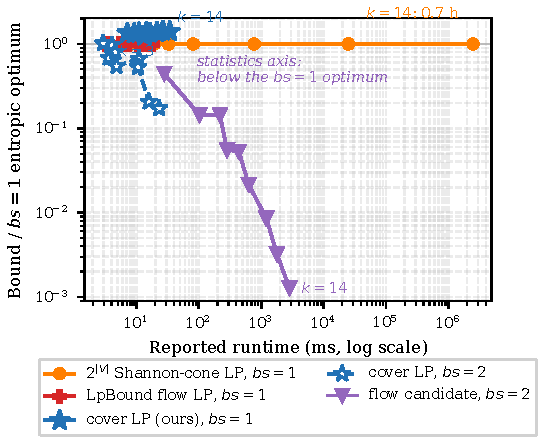
\includegraphics[width=\columnwidth]{positioning.pdf}
\caption{Both axes on one \emph{measured} cost--tightness plot (each
point a synthetic cycle-$k$ query; $y$ is relative to the entropic
optimum on single-relation statistics). Above $y{=}1$, the inference
axis at $bs{=}1$: CEG$_M$/PANDA is cheap but up to $45\times$ loose,
the cover LP within $1.3\times$ ($7$--$46$\,ms end to end), and the
optimum itself $43$\,s at $k{=}12$ as a $2^{|V|}$ program but a
$3$--$18$\,ms solve ($k{\le}14$) as LpBound's flow LP---that axis is
closed. Below $y{=}1$, the statistics
axis: the same programs on $bs{=}2$ block statistics, the cover LP level
with the optimum at $k{\le}4$ and up to $6\times$ below it, the flow LP
(Section~\ref{sec:scalability}) $2$--$800\times$ below. Data: \texttt{scale\_entropic.csv},
\texttt{flow\_scale.csv}, \texttt{baseline\_comparison.csv}.}
\label{fig:positioning}
\end{figure}

Our contributions are:

\begin{enumerate}
\item \textbf{On single-relation statistics the inference axis is closed
(Section~\ref{sec:vs-lpbound}).}
On a fixed hyperpath the cover LP is optimal over \emph{every} valid
weight vector: a cutting-plane search adding Shannon cuts to a
relaxation converges back to exactly the cover bound. The gap to the
entropic optimum comes from statistics the hyperpath leaves unused, not
from the weighting---and LpBound's flow LP, which uses them, reaches that
optimum in polynomial time, so at $bs{=}1$ the cover LP is dominated as a
bound.

\item \textbf{The statistics axis is open
(Section~\ref{sec:stats-vs-inference}).}
Block statistics $\mu_p(\block \mid \interface)$, $|\block|\ge2$, are
worth a median $56\times$ on the $109$ short cycles of a pre-registered
Hetionet suite (rows capped at $3$K) and $80$--$2{,}500\times$ on $120/120$
longer Hetionet cycles ($|V|{=}6$--$10$), against a median
$2.5$--$3.6\times$ of inference headroom. On $120$ IMDb cycles from
JOB's snapshot the margin is smaller: $4$--$43\times$ with the cover LP
($17$--$177\times$ with the flow LP) against $3.8$--$4.3\times$, level at
$|V|{=}6$. On homogeneous synthetic cycles the axes are comparable.

\item \textbf{Richer statistics reopen the program
(Sections~\ref{sec:stats-vs-inference},~\ref{sec:scalability}).}
On the same block statistics the polymatroid optimum beats the cover LP
by $1.5$--$3.8\times$ ($12/12$ synthetic) and a median $3.2$--$5.1\times$
(Hetionet), against $1.15$--$1.5\times$ on single-relation statistics;
on IMDb it stays level at $200$ films ($3.3$--$4.2\times$) and grows to
$6.8\times$ at $1{,}000$.
Extending Im et al.'s flow LP to $\ell_p$ block constraints reaches that
optimum in polynomial time on $12/12$ synthetic instances, every synthetic
even cycle to $k{=}10$ and $189/240$ real-data queries ($0.03$--$4.4$\,s at
$k{=}3$--$16$).

\item \textbf{Which block statistic matters
(Section~\ref{sec:stats-vs-inference}).}
Under the same program (the order-relaxed flow LP, so a lower bound on
the gain), block statistics carry
a further median $63\times$ on Hetionet beyond pair-join sizes, a proxy
for the two-relation statistic CorrBound adds (itself worth $31\times$
there; on IMDb, where half the pairs are self-joins, sizes add almost nothing). For a block of two binary relations all but one of them come from
single-relation passes; the exception, the $\ell_2$ norm of the
common-neighbour counts, restores the full bound on $85/120$ Hetionet and
$116/120$ IMDb queries.

\item \textbf{Validity, cost and limits
(Sections~\ref{sec:theory},~\ref{sec:experiments},~\ref{sec:wcoj}).}
An $\ell_p$ Composition Inequality makes the cover bound valid for every
hyperpath, block size and $p$; the proof turns redundant coverage into a
fractional cover, and $207$K databases plus an LP certificate over
$6{,}197$ hyperpath structures independently agree. Block statistics cost a median $45\times$ more to
collect, once per database; cataloged on Hetionet, a $bs{=}2$ estimate costs
$10$\,ms. Guiding join order, the bound trims the catastrophic tail on
synthetic cliques (P95 slowdown $1.2\times$ vs.\ $5.8\times$) rather than
the average, and on IMDb block statistics pick the exact-count order on
$24/40$ queries, yet those left-deep plans still lose to DuckDB's own; and a
per-step residual ordering heuristic does not generalize (median
$-1.3\%$ over $66$ queries).
\end{enumerate}

%% ===================================================================
\section{Preliminaries}
\label{sec:prelim}

\subsection{Query Hypergraphs}

A conjunctive query $\query$ over relations $\rel_1, \ldots, \rel_m$
with attributes $V = \{a_1, \ldots, a_n\}$ is represented as a
hypergraph $H = (V, \mathcal{E})$ where each hyperedge $e_i \in
\mathcal{E}$ corresponds to the attribute set of relation $\rel_i$.
The full natural join is $\query = \bowtie_{i=1}^{m} \rel_i$.

\subsection{CEG and MOLP}

Cardinality Estimation Graphs~\cite{chen2022ceg,salihoglu2026ceg} model
both optimistic and pessimistic estimators as path-finding in a directed
graph.
The pessimistic CEG$_M$ uses max-degree edge weights: for relation
$\rel$ with interface $\interface$,
$\muFactor{\rel}{\interface} = \max_{a_\interface}
|\ext{\rel}{a_\interface}|$.
The MOLP bound~\cite{joglekar2016molp} equals the minimum-weight path
in CEG$_M$.

\subsection{Block Extensions and Hyperpaths}

A \emph{block} $\block \subseteq \mathcal{E}$ is a connected subset
of relations.
The \emph{block extension factor}~\cite{hceg2027} is
$\muFactor{\block}{\interface} = \max_{a_\interface}
|\ext{\block}{a_\interface}|$,
where $\interface = \attr{\joinstate} \cap \attr{\block}$ is the
interface with the current state.
A \emph{hyperpath} $P = (\joinstate_0{=}\emptyset, \block_1,
\joinstate_1, \ldots, \block_m, \joinstate_m{=}\mathcal{E})$
decomposes the query into sequential block extensions.
The product $\prod_{j=1}^{m} \muFactor{\block_j}{\interface_j}$ is
a valid cardinality upper bound (Composition
Lemma~\cite{hceg2027}).
Our framework generalizes this product by replacing $\ell_\infty$
norms with LP-optimized $\ell_p$-norms.

\subsection{LpBound: $\ell_p$-Norm Degree Sequences}

LpBound~\cite{zhang2025lpbound} uses $\ell_p$-norms of degree
sequences as tighter statistics.
For relation $\rel$ with degree sequence
$\mathbf{d} = (d_1, \ldots, d_k)$ where
$d_i = |\ext{\rel}{a_i}|$, the $\ell_p$-norm is
$\lpnorm{\mathbf{d}}{p} = (\sum_i d_i^p)^{1/p}$.
The core inequality is: for any $p \ge 1$,
\[
\tfrac{1}{p}\, h(U) + h(V \mid U) \le \log \lpnorm{\mathbf{d}}{p}
\]
where $h$ denotes entropy.
Optimizing over all valid inequalities via an LP yields bounds
orders of magnitude tighter than max-degree alone.

%% ===================================================================
\section{LpH-CEG Framework}
\label{sec:framework}

\subsection{$\ell_p$-Norm Block Extension Factor}

\begin{definition}[$\ell_p$ Block Extension Factor]
\label{def:lp-mu}
For a block $\block$ with interface $\interface$, let
$\mathbf{d} = (d_1, \ldots, d_k)$ be the degree sequence where
$d_i = |\ext{\block}{a_i}|$ for each distinct interface value
$a_i \in \pi_\interface(\query_\block)$.
The $\ell_p$ block extension factor is:
\[
\muLp{p}{\block}{\interface} = \lpnorm{\mathbf{d}}{p}
= \Bigl(\sum_{i=1}^{k} d_i^p\Bigr)^{1/p}
\]
\end{definition}

\noindent Special cases:
$\muLp{\infty}{\block}{\interface} = \max_i d_i = \muFactor{\block}{\interface}$ (max-degree);
$\muLp{1}{\block}{\interface} = \sum_i d_i = |\query_\block|$ (cardinality).

\subsection{Fractional Block Cover LP}

Given a hyperpath $P$ with $m$ steps, we define a variable
$w_{j,p} \ge 0$ for each step $j$ and each $p$-value.
The LP minimizes the log-space bound:

\begin{equation}
\label{eq:lp}
\min \sum_{j=1}^{m} \sum_{p \in \mathcal{P}}
w_{j,p} \cdot \log_2 \muLp{p}{\block_j}{\interface_j}
\end{equation}

subject to the fractional block cover constraints: for each
attribute $a \in V$,
\begin{equation}
\label{eq:cover}
\sum_{p \in \mathcal{P}}\;\Biggl(
\sum_{\substack{j:\, a \in \attr{\block_j} \setminus \interface_j}}
\!\!\! w_{j,p}
\;+\;
\sum_{\substack{j:\, a \in \interface_j}}
\frac{w_{j,p}}{p}
\Biggr)
\;\ge\; 1
\end{equation}

The LP has $O(m \cdot |\mathcal{P}|)$ variables and $|V|$ constraints,
solvable in one to two milliseconds for typical queries.

\subsection{Why Cyclic Queries Benefit}

\begin{proposition}[Acyclic rigidity]
\label{prop:acyclic}
For an acyclic hyperpath with binary extensions ($|\block_j| = 1$),
every attribute is new at exactly one step. No attribute is then covered
twice as an \emph{extension}, so no step's weight can be reduced by
another step's extension term, and on star queries the LP returns
$w_j = 1$ throughout, recovering the max-degree bound. It does not
follow that every acyclic weight is $\ge 1$: a later step may cover an
attribute through its \emph{interface} at $p=1$, and on a $4$-path the
LP returns $(1, 0, 1)$. See Section~\ref{sec:noimprove} for what this
does and does not buy.
\end{proposition}

\begin{proposition}[Cyclic slack]
\label{prop:cyclic}
In a cycle of length $k$ with binary extensions, the cycle-closing
attribute appears in $\ge 2$ steps (as extension in one, interface in
another).
The cover constraint allows distributing weight across these steps,
enabling $w_j < 1$ and intermediate $\ell_p$-norms.
\end{proposition}

\subsection{Algorithm}

Algorithm~\ref{alg:lph-ceg} summarizes the LpH-CEG estimation pipeline.

\begin{algorithm}[t]
\caption{LpH-CEG Estimation}
\label{alg:lph-ceg}
\begin{algorithmic}[1]
\REQUIRE Query hypergraph $H$, relation data $D$, block size limit $b$,
  $p$-values $\mathcal{P} = \{p_1, \ldots, p_r\}$
\ENSURE Upper bound $\hat{C}$ on $|\query(D)|$
\STATE Enumerate blocks $\mathcal{B} \gets \{F \subseteq \mathcal{E} :
  |F| \le b,\; F \text{ connected}\}$
\FOR{each block $F \in \mathcal{B}$ and interface $I$}
  \STATE Compute join $Q_F \gets \bowtie_{R \in F} R$
  \STATE Collect degree sequence $\mathbf{d}_{F,I}$
  \STATE Compute $\muLp{p}{F}{I}$ for each $p \in \mathcal{P}$
\ENDFOR
\STATE Build block-extension DAG with $\ell_\infty$ weights
\STATE Find $K$ shortest hyperpaths $P_1, \ldots, P_K$ \COMMENT{$K{=}1$: default}
\FOR{each hyperpath $P_i = (F_1, \ldots, F_m)$}
  \STATE Solve LP~\eqref{eq:lp}--\eqref{eq:cover} for weights $(w^*_{j,p})$
  \STATE $\hat{C}_i \gets \prod_{j,p} \muLp{p}{F_j}{I_j}^{\,w^*_{j,p}}$
\ENDFOR
\STATE \textbf{return} $\min(\hat{C}_1, \ldots, \hat{C}_K,\; \text{max-deg bound})$
\end{algorithmic}
\end{algorithm}

The LP in line~10 has $O(m \cdot |\mathcal{P}|)$ variables
($m \le n$ steps, $|\mathcal{P}| = 3$ in practice) and $n$
constraints.
We solve it via HiGHS~\cite{huangfu2018highs} in $<1$\,ms for all
queries in our experiments.
Line~13 ensures LpH-CEG never produces a looser bound than the
standard max-degree bound.

%% ===================================================================
\section{Theoretical Results}
\label{sec:theory}
Proofs not given in full here are in the extended version shipped with
the artifact.

\begin{theorem}[$\ell_p$ Composition Inequality]
\label{thm:composition}
Let $P = (\joinstate_0{=}\emptyset, \ldots, \joinstate_m{=}\mathcal{E})$
be a hyperpath, and let $(w_{j,p})$ satisfy the cover
constraint~\eqref{eq:cover}.
Then:
\[
|\query| \le \prod_{j=1}^{m} \prod_{p \in \mathcal{P}}
\muLp{p}{\block_j}{\interface_j}^{\,w_{j,p}}
\]
\end{theorem}

\begin{proof}
Let $h$ be the entropy of the uniform distribution on $\query(D)$, so
$h(V)=\log_2|\query|$. Write $A_j=\attr{\block_j}$,
$V_j=\attr{\joinstate_j}$ and $E_j=A_j\setminus\interface_j$: the $E_j$
partition $V$ and $\interface_j\subseteq V_{j-1}$. Since
$\pi_{A_j}\query\subseteq\bowtie_{\rel\in\block_j}\rel$, the $\ell_p$
inequality of~\cite{abokhamis2024lpnorm} gives
$\frac1p h(\interface_j)+h(E_j\mid\interface_j)\le
\log_2\muLp{p}{\block_j}{\interface_j}$. Weight by $w_{j,p}$ and sum; with
$w_j=\sum_p w_{j,p}$ and $s_j=\sum_p w_{j,p}/p$ it remains to show
$\sum_j[s_jh(\interface_j)+w_jh(E_j\mid\interface_j)]\ge h(V)$, where
\eqref{eq:cover} reads $w_{j(a)}+\sum_{j':a\in\interface_{j'}}s_{j'}\ge1$
for the step $j(a)$ that binds $a$. Let $g_j=h(E_j\mid V_{j-1})$ and
$\delta_j=\max(0,1-w_j)$. (i)~By the chain rule and submodularity,
$h(\interface_{j'})\ge\sum_j h(\interface_{j'}\cap E_j\mid V_{j-1})$.
(ii)~If $\delta_j>0$, \eqref{eq:cover} makes
$\{\interface_{j'}\cap E_j\}$, weighted $s_{j'}/\delta_j$, a fractional
cover of $E_j$; $S\mapsto h(S\mid V_{j-1})$ is monotone submodular, hence
fractionally subadditive, so
$\sum_{j'}s_{j'}h(\interface_{j'}\cap E_j\mid V_{j-1})\ge\delta_jg_j$.
(iii)~As $\interface_j\subseteq V_{j-1}$,
$w_jh(E_j\mid\interface_j)\ge(1-\delta_j)g_j$. Summing gives at least
$\sum_jg_j=h(V)$.
\end{proof}

Only monotonicity and submodularity are used, so the argument holds over
the whole polymatroid cone. The redundant coverage that lets per-step
weights fall below $1$---the source of every cyclic improvement, and the
reason the elementary per-step argument ($w_j\ge1$) does not apply---enters
exactly as the fractional cover in~(ii). The theorem assumes exact
statistics of the database being bounded; the sketched $\ell_2$ of
Section~\ref{sec:stats-vs-inference} is outside it.

\paragraph{Independent checks.} Two checks that do not rely on the proof
agree with it. Over $207{,}000$ databases---every database over a
two-value domain for the triangle and $4$-cycle, plus $15{,}000$ random
ones across six shapes at block sizes $1$--$3$---the estimate never fell
below the exact count (minimum ratio $1.0$). And because the remaining
inequality is linear in $h$ and affine in $w$, an LP over the polymatroid
cone decides it for every vertex of the feasible weight region: across
$6{,}197$ hyperpath structures on eleven shapes with $|V|\le6$ and block
sizes $1$--$3$ ($1.73$M vertices; every hyperpath on $19$ of the $33$
(shape, block size) pairs) the minimum slack is exactly $0$---tight,
never negative. Both ship as regression gates.

\begin{theorem}[Subsumption]
\label{thm:subsumption}
LpH-CEG subsumes:
\begin{enumerate}
\item Max-degree block bounds~\cite{hceg2027}: setting $p = \infty$,
  $w_j = 1$ recovers the Composition Lemma.
\item Binary $\ell_p$-cover bounds: setting $|\block_j| = 1$ recovers
  the fractional $\ell_p$-cover over single relations---a polynomial-size
  relaxation of LpBound's~\cite{zhang2025lpbound} entropic LP
  (Section~\ref{sec:vs-lpbound}), not necessarily its entropic optimum.
\item AGM bound~\cite{atserias2008agm}: setting $p = 1$ on every step
  makes each attribute's coverage $1$ per covering step, so~\eqref{eq:cover}
  becomes the fractional edge-cover constraint and the objective becomes
  $\prod_j |\rel_j|^{w_j}$.
\end{enumerate}
\end{theorem}

\subsection{Relationship to LpBound}
\label{sec:vs-lpbound}

LpBound~\cite{zhang2025lpbound} also applies to cyclic queries and also
solves a linear program over $\ell_p$-norm degree statistics, so we must
delineate precisely what the block-cover LP adds.

\paragraph{Two different LPs.}
LpBound's bound is the optimum of an \emph{entropic} LP: it maximizes
$h(V)$ over the Shannon cone---monotonicity and submodularity
inequalities on all $2^{|V|}$ entropic terms---subject to the
$\ell_p$-norm statistics constraints, and is provably the tightest bound
those statistics admit~\cite{zhang2025lpbound,abokhamis2024lpnorm}.
Our LP~\eqref{eq:lp}--\eqref{eq:cover} instead optimizes
$O(m\,|\mathcal{P}|)$ weights over a \emph{fixed hyperpath}, with one
fractional-cover constraint per attribute.
On identical statistics the entropic optimum is the tighter of the two by
construction, and we do not claim otherwise: at $bs{=}1$ the cover bound
is $1.25$--$1.43\times$ looser on synthetic power-law cycles
(Figure~\ref{fig:crossover}), $1.9$--$3.5\times$ on six hand-picked
real Hetionet cycles (\texttt{baseline\_comparison.csv}), and up to $8.8\times$ on one
relation repeated along a long chain, where the entropic cone exploits
conditional structure the fixed hyperpath treats independently.

\paragraph{On a fixed hyperpath, reweighting is exhausted.}
Could a better weighting of the hyperpath's statistics close that gap?
No.
Since the remaining inequality is affine in $w$, one can minimize over a relaxation of the
valid-weight set, test the minimizer with the polymatroid LP, and add
the violating $h$ as a cut. Run to convergence on triangle,
cycle-$4$/$5$/$6$ and $K_4$, this returns \emph{exactly} the cover
bound (cycle-4: $15.335$ in $\log_2$, against $14.858$ entropic). On a
fixed hyperpath the cover LP is already optimal over every valid weight
vector; the residual gap comes from \emph{statistics} the hyperpath
leaves unused, which the entropic program exploits and
Section~\ref{sec:stats-vs-inference} extends.

\emph{The gap is predictable:} over $198$ configurations four structural
features give a held-out $R^2$ of $0.87$, and higher skew shrinks it (gap
$\to 1$ by $\alpha{=}3$; $\rho{=}{-}0.74$).

\paragraph{Efficiency, stated correctly.}
The Shannon-cone \emph{formulation} of that optimum has $2^{|V|}$
variables and $O(2^{|V|}|V|^2)$ constraints and degrades accordingly:
$111$\,ms at $|V|{=}8$, $43$\,s at $|V|{=}12$, $\sim$1\,h at $|V|{=}14$,
unsolvable beyond (Figure~\ref{fig:crossover}; the same curve on real
Hetionet degree sequences: $46$\,s and $39$\,min). But that is not what
LpBound solves. Its LPflow~\cite[Thm.~4.5]{zhang2025lpbound} rewrites
every simple $\ell_p$ constraint (one conditioning attribute) as a flow
bundle after Im et al.~\cite{im2025simple} and is polynomial; our
reimplementation returns the entropic bound to $10^{-6}$ on every
instance we compared (12 families, the sweep, the 240 long-suite queries) in $3$--$26$\,ms at $k{=}3$--$16$
(Figure~\ref{fig:crossover}). So at $bs{=}1$ the cover LP buys
\emph{no} asymptotic advantage over LpBound, and we withdraw that
reading: as a $bs{=}1$ bound the cover LP is dominated---looser, and
both solve in milliseconds. The fixed hyperpath buys the per-step decomposition
(item~1) and the framework the statistics vocabulary (item~2), where
inference becomes non-trivial again (Section~\ref{sec:scalability}).

\paragraph{What the block-cover LP adds.}
Not size or speed. What LpBound's single global program does not provide
is structural:
\begin{enumerate}
\item \textbf{A per-step residual bound.} Because the LP is attached to
  a hyperpath, it yields a bound \emph{per extension step}, and hence a
  residual bound for any variable prefix. This is exactly the signal our
  WCOJ variable ordering consumes (Section~\ref{sec:wcoj}); LpBound's
  single global optimum exposes no such per-step decomposition.
\item \textbf{Block-level statistics.} With multi-way blocks
  ($|\block_j| > 1$) the LP draws on $\ell_p$-norms of \emph{joined}
  block relations---statistics outside LpBound's single-relation
  vocabulary.
\end{enumerate}
So at $bs{=}1$ LpH-CEG trades a little tightness for a decomposable
bound; item~2 is the axis the paper is about
(Section~\ref{sec:stats-vs-inference}).

\begin{theorem}[Cyclic Improvement]
\label{thm:cyclic}
Consider a cycle query $C_k$ ($k \ge 3$) evaluated by binary
extensions in cycle order, where relation $R_j$ has cardinality
$N_j = |R_j|$, maximum degree $M_j$, and degree-sequence
$\ell_p$-norms $\mu_p(R_j)$.
Then:
\begin{enumerate}
\item \textbf{(Standard bound.)} The max-degree bound is
\[
B_{\max} = N_1 \prod_{j=2}^{k-1} M_j ,
\]
where the first extension has empty interface and contributes the
cardinality $N_1$, the $k-2$ \emph{middle} extensions each contribute
a max-degree $M_j$, and the cycle-closing extension (interface of size
two, empty extension set) contributes a factor of $1$.
\item \textbf{(LP bound.)} For every $p \ge 1$ the fractional
block-cover LP~\eqref{eq:lp}--\eqref{eq:cover} is feasible with weight
$p/(p{+}1)$ and exponent $p$ on every middle extension, together with
the split $(\frac{p}{p+1}, \frac{1}{p+1})$ of unit weight across the first
and closing ($\ell_1$) extensions. This yields
\[
B_{\mathrm{LP}} \le \min_{p \ge 1}\; N_1^{\frac{p}{p+1}} N_k^{\frac{1}{p+1}}
\prod_{j=2}^{k-1} \mu_p(R_j)^{\frac{p}{p+1}} ,
\]
e.g.\ $N_1^{2/3} N_k^{1/3} \prod_j \mu_2(R_j)^{2/3}$ at $p{=}2$. (The
exponent must be common, or non-increasing along the cycle: the cover
constraint of the attribute between edges $j$ and $j{+}1$ reads
$\frac{p_j}{p_j+1} + \frac{1}{p_{j+1}+1} \ge 1$.)
\item \textbf{(Improvement.)} Therefore, for every $p \ge 1$,
\[
\frac{B_{\max}}{B_{\mathrm{LP}}} \;\ge\;
\Bigl(\frac{N_1}{N_k}\Bigr)^{\!\frac{1}{p+1}}
\prod_{j=2}^{k-1}
\frac{M_j}{\mu_p(R_j)^{\,p/(p+1)}} .
\]
At $p{=}2$ each middle factor exceeds $1$ when the relation is skewed
($\mu_2(R_j) < M_j^{3/2}$); as $p \to \infty$ every factor tends to $1$.
The boundary factor is a constant independent of $k$;
for a \emph{uniform} cycle ($N_j \equiv N$) it equals $1$, and in the
general case it can be made $\ge 1$ by entering the cycle at the largest
relation ($N_1 \ge N_k$). The improvement is therefore dominated by the
product of $k-2$ per-edge factors and grows geometrically in the number
of middle edges $k-2$. Since LpH-CEG returns
$\min(B_{\max}, B_{\mathrm{LP}})$, the realized ratio is always
$\ge 1$.
\end{enumerate}
\end{theorem}

\begin{proof}[Proof sketch]
The standard bound (1) follows directly from the cycle hyperpath
structure: the first extension has empty interface, so its degree
sequence is the single value $N_1$ and $\mu_\infty = N_1$; each middle
extension adds one attribute over a size-one interface with
$\mu_\infty = M_j$; the closing extension has both endpoints already in
the state, so its conditional degrees are all $1$ and $\mu_\infty = 1$.
For (2), each attribute is covered as an extension in one step (rate
$1$) and as an interface in the next (rate $1/p$); with a common $p$ the
local constraint $w + w/p \ge 1$ is tight at $w = p/(p+1)$. Attribute
$a_2$ then reads $w_1 + \frac{1}{p+1} \ge 1$, $a_k$ reads
$\frac{p}{p+1} + w_k \ge 1$ and $a_1$ reads $w_1 + w_k \ge 1$, all tight
at $w_1 = \frac{p}{p+1}$, $w_k = \frac{1}{p+1}$. The closing step has
$\mu_1 = N_k$, so the first/closing contributions are
$N_1^{p/(p+1)} N_k^{1/(p+1)}$ against $N_1$ in $B_{\max}$. The LP optimum
is at most every such point, and may mix $p$ further.
\end{proof}

\begin{corollary}[Scalability with cycle size]
\label{cor:scalability}
For cycle-$k$ queries on power-law graphs with fixed parameters,
the LpH-CEG improvement ratio grows exponentially with $k$.
Our experiments confirm (10-seed mean):
$8.4\times$ ($k{=}4$), $69\times$ ($k{=}6$),
$614\times$ ($k{=}8$).
\end{corollary}

\subsection{Tightness and Limitations}

Theorem~\ref{thm:composition} establishes that LpH-CEG bounds are
\emph{valid} (never underestimate), but not necessarily \emph{tight}
(matching a worst-case instance).
Tightness depends on the degree sequence structure:

\begin{proposition}[Per-step tightness]
\label{prop:tightness}
Each step's $\ell_p$ inequality is tight when its interface is simple
($|\interface_j| \le 1$)~\cite{abokhamis2024lpnorm}. Under binary
extensions most interfaces are simple, the exceptions being the first
step ($\interface_1 = \emptyset$) and any closing step, whose interface
carries the two endpoints of the closing edge.
\end{proposition}

Per-step tightness does not make the \emph{composition} tight: the
weighted product can be loose even where every factor is exact, and we
measure it to be $1.25$--$8.8\times$ looser than the entropic optimum at
$bs{=}1$ (Section~\ref{sec:vs-lpbound}).

This creates a principled trade-off: binary extensions keep simple
interfaces; multi-way blocks capture block-level correlation at the cost
of non-simple ones. Results use $bs{=}1$ unless marked $bs{=}2$.

\subsection{Delta over the Block Framework}

We inherit the block-extension DAG and hyperpath machinery from
H-CEG~\cite{hceg2027}, which uses only $\ell_\infty$ weights with no
optimization layer. What this paper adds is the $\ell_p$ fractional cover
LP that replaces those fixed scalars, the separation of the statistics and
inference axes (Section~\ref{sec:stats-vs-inference}), the flow-LP
inference over block statistics (Section~\ref{sec:scalability}), and
the per-step residual signal; none exists in H-CEG. Theorem~\ref{thm:cyclic}
additionally supplies a structural test neither predecessor provides,
predicting the magnitude from a product of $k-2$ per-edge factors
$M_j / \mu_p(\rel_j)^{p/(p+1)}$ at a common $p$.

%% ===================================================================
\section{WCOJ Variable Ordering}
\label{sec:wcoj}

LpH-CEG bounds naturally guide WCOJ variable ordering.
At each step of the greedy ordering, we select the variable whose
removal minimizes the LP-optimized residual bound
(Algorithm~\ref{alg:ordering}):

\begin{algorithm}[t]
\caption{LpH-CEG Variable Ordering for WCOJ}
\label{alg:ordering}
\begin{algorithmic}[1]
\REQUIRE Query $H$, relation data $D$
\ENSURE Variable ordering $\sigma = (v_1, \ldots, v_n)$
\STATE $\sigma \gets []$, $\text{chosen} \gets \emptyset$
\FOR{$i = 1$ \TO $n$}
  \FOR{each $v \in V \setminus \text{chosen}$}
    \STATE $b_v \gets \text{LpH-CEG-Bound}(H|_{V \setminus
      (\text{chosen} \cup \{v\})}, D)$
  \ENDFOR
  \STATE $v^* \gets \arg\min_v b_v$
  \STATE Append $v^*$ to $\sigma$; add $v^*$ to chosen
\ENDFOR
\end{algorithmic}
\end{algorithm}

On the Hetionet cycle-4 query, the LP-guided ordering
(gene1$\to$gene2$\to$compound$\to$disease) differs from the
standard max-degree ordering
(compound$\to$disease$\to$gene2$\to$gene1) and reduces
GenericJoin iterations from $2{,}765{,}886$ to $1{,}209{,}687$---a
$2.3\times$ reduction (a deterministic, machine-independent metric)
resulting in $2.6\times$ faster wall-clock execution in our simulator.

\paragraph{Does it generalize? An honest negative.}
It does not, and we report this plainly. On a broad synthetic suite
($66$ queries across seven shapes, two sizes, two skews, and three
seeds; joins too large to enumerate are censored), the LP-residual
ordering is \emph{not} a general improvement over the max-degree
(H-CEG) residual ordering: the median iteration ratio is $0.99$
($-1.3\%$), it wins on $20$ queries but loses on $43$ (Wilcoxon
$p{=}0.003$, Cliff's $\delta{=}{-}0.35$), and its $90$th-percentile
regression is $1.8\times$. The Hetionet win reflects a regime
(heterogeneous relations with asymmetric skew), not a universal effect,
so we treat LP-guided ordering as a targeted heuristic, not a systems
contribution (see also Section~\ref{sec:robustness}).

%% ===================================================================
\section{Experimental Evaluation}
\label{sec:experiments}

\subsection{Setup}

\paragraph{Datasets.}
We evaluate on three real-world datasets:
\textbf{Hetionet}~\cite{himmelstein2017hetionet} (biomedical knowledge graph,
45K nodes, 2M edges, heterogeneous);
\textbf{Epinions} (social network, 75K nodes, 509K edges);
\textbf{IMDb}, JOB's snapshot~\cite{leis2015goodare}: the $200$
most-voted feature films for a cycle suite, and the JOB-medium subset.
We also use synthetic power-law graphs (100--5{,}000 nodes,
400--20{,}000 edges).
All synthetic experiments report mean $\pm$ std over 10 random seeds.

\paragraph{Queries.}
Synthetic cycle-$k$ for $k \in \{3,\ldots,16\}$ plus diamond and $K_4$ families;
on real data, three registered suites
(Section~\ref{sec:suite}) plus a handful of hand-picked cycles.

\paragraph{Baselines.}
AGM (fractional edge cover, $\prod |R_i|^{w_i}$);
CEG$_M$ (binary max-degree shortest path, $bs{=}1$; equivalent
to PANDA/MOLP on binary queries~\cite{abokhamis2017panda,joglekar2016molp});
LpH-CEG (LP-optimized $\ell_p$-norms,
$\mathcal{P} = \{1,2,\infty\}$).
The ``LpH-CEG'' column throughout denotes our
\emph{cover}-LP at $bs{=}1$ (Section~\ref{sec:vs-lpbound}); it is
\emph{not} the entropic LpBound of
Zhang et al.~\cite{zhang2025lpbound}, against which we compare
separately in Section~\ref{sec:vs-lpbound} (our cover bound is
$1.3\times$ looser on synthetic cycles, up to ${\sim}9\times$ on
homogeneous real chains).
Learned and summary estimators (FactorJoin, GNCE,
COLOR~\cite{deeds2025color,schwabe2024gnce}) produce \emph{point}
estimates without guaranteed upper bounds; CorrBound, which enriches the
entropic program with cross-relation statistics, is compared through a
proxy in Section~\ref{sec:stats-vs-inference}.

\paragraph{Unified bound comparison.}
Table~\ref{tab:baselines} places all four guaranteed-bound methods on one
suite. The ordering is as predicted: CEG$_M \ge$ Cover-LP $\ge$ Entropic,
with AGM incomparable (it ignores degrees). Our cover-LP is
$2.3$--$35.7\times$ tighter than CEG$_M$ on synthetic cycles, is also
consistently tighter than AGM (e.g.\ $2.0\times$ on cycle-6), and stays
within $1.25$--$1.36\times$ of the entropic optimum---the best any
$\ell_p$-statistics bound can achieve.

\begin{table}[t]
\centering
\caption{Unified comparison of guaranteed upper bounds (synthetic
power-law cycles, $100$V/$400$E). ``Cover'' is our $bs{=}1$ LP;
``Entropic'' is the $2^{|V|}$ LpBound. Lower is tighter.
``$/$CEG'' and ``$/$Ent'' are Cover's ratio to CEG$_M$ and to the
entropic optimum.}
\label{tab:baselines}
\begin{tabular}{@{}lrrrrrr@{}}
\toprule
Query & AGM & CEG$_M$ & Cover & Entropic & $/$CEG & $/$Ent \\
\midrule
Cycle-3 & 8.0K & 15.6K & 6.8K & 5.0K & $2.3\times$ & $1.36\times$ \\
Cycle-4 & 160K & 655K & 116K & 87K & $5.7\times$ & $1.32\times$ \\
Cycle-5 & 3.2M & 25.5M & 1.97M & 1.45M & $13.0\times$ & $1.36\times$ \\
Cycle-6 & 64M & 1.12B & 31.5M & 25.2M & $35.7\times$ & $1.25\times$ \\
\bottomrule
\end{tabular}
\end{table}

\subsection{Main Results: Cyclic Query Bounds}

\begin{table}[t]
\centering
\caption{LpH-CEG vs.\ CEG$_M$ on synthetic cycle queries ($bs{=}1$,
$|V|{=}200$, $|E|{=}800$, mean $\pm$ std over 10 seeds).
The ratio is a \emph{bound-tightening} measure (CEG$_M$/LpH-CEG); the
$q$-error column (accuracy vs.\ the true count) is shown only where the
exact count is feasible to materialize, and is ``---'' for $k \ge 6$
where the true cardinality is intractable to compute.}
\label{tab:synthetic}
\begin{tabular}{@{}lrrrl@{}}
\toprule
Query & CEG$_M$ & LpH-CEG & Ratio & $q$-error \\
\midrule
Cycle-3 &  53K$\pm$2K  &  19K$\pm$0.3K & $2.75{\pm}0.13\times$ & 10.8$\pm$0.2$\times$ \\
Cycle-4 & 3.8M$\pm$253K & 448K$\pm$44K & $8.43{\pm}0.78\times$ & 18.3$\pm$1.8$\times$ \\
Cycle-5 & 270M$\pm$18M  & 11.3M$\pm$308K & $23.8{\pm}1.3\times$ & 39.0$\pm$1.1$\times$ \\
Cycle-6 & 18.8B$\pm$2.3B & 272M$\pm$16M & $68.9{\pm}6.4\times$ & --- \\
Cycle-7 & 1.4T$\pm$167B & 6.5B$\pm$329M & $211{\pm}20\times$ & --- \\
Cycle-8 & 97T$\pm$14T  & 158B$\pm$10B & $\mathbf{614{\pm}71\times}$ & --- \\
\bottomrule
\end{tabular}
\end{table}

Table~\ref{tab:synthetic} shows the core result: LpH-CEG achieves
$2.8\times$ to $614\times$ tighter bounds than CEG$_M$ on cyclic
queries, with tight standard deviations (relative std $< 12\%$)
confirming stability across random graph instances.
The improvement \emph{scales with cycle size}: from $8.4\times$
on cycle-4 to $69\times$ on cycle-6 to $614\times$ on cycle-8.
It also \emph{scales with data size}: cycle-4 improves from $5.9\times$
(100V) to $34\times$ (2KV), with the dependence on skew characterized in
Section~\ref{sec:jobskew}.

\subsection{Statistics Versus Inference}
\label{sec:stats-vs-inference}

The two axes can be separated directly: hold the program fixed and change
the statistics, then hold the statistics fixed and change the program.
Table~\ref{tab:stats-vs-inf} is that $2{\times}2$, over four families and
three seeds, with the exact join size computed so every bound is checked
rather than assumed.

\begin{table}[t]
\centering
\caption{Statistics $\times$ inference, $40$ vertices / $120$ edges,
seed $101$ (12 family--seed pairs behave alike; see text). Both programs
see the same catalog: every single relation, or every $bs{\le}2$
block and interface. Every entry is a valid upper bound on the exact
count.}
\label{tab:stats-vs-inf}
\begin{tabular}{@{}lrrrr@{}}
\toprule
 & \multicolumn{2}{c}{cover LP} & \multicolumn{2}{c}{polymatroid optimum} \\
\cmidrule(lr){2-3}\cmidrule(lr){4-5}
Query & single & block & single & block \\
\midrule
Triangle & 1{,}083 & 668  & 806   & $\mathbf{368}$ \\
Cycle-4  & 9{,}871 & 4{,}716 & 7{,}436 & $\mathbf{1{,}355}$ \\
Diamond  & 9{,}769 & 4{,}560 & 7{,}436 & $\mathbf{1{,}355}$ \\
\bottomrule
\end{tabular}
\end{table}

Reading the table by column pairs gives the central observation. At fixed
program, the statistics axis (single $\to$ block) improves the bound by
$1.5$--$2.3\times$ for the cover LP and $1.7$--$5.5\times$ for the
optimum; at fixed statistics, the inference axis (cover $\to$ optimum)
improves it by $1.15$--$1.5\times$ on single-relation statistics and
$1.5$--$3.8\times$ on block ones, over all 12 pairs. The axes interact:
richer statistics give the program more to exploit. The statistics axis
has room because a block statistic $\mu_p(\block \mid \interface)$ with
$|\block| \ge 2$ describes a multi-relation join, which no
single-relation degree \emph{sequence} determines (most of it follows
from single-relation degree \emph{tables}; see below).

Two scoping points keep this from being overstated, both measured on the
headline cycle protocol ($|V|{=}200$, $|E|{=}800$, 10 seeds) so the axes
are in the same units:

\begin{center}\small
\begin{tabular}{@{}lrrr@{}}
\toprule
Axis & cycle-4 & cycle-6 & cycle-8 \\
\midrule
inference: max-deg $\to$ cover LP & $8.8\times$ & $72.7\times$ & $654\times$ \\
inference: cover LP $\to$ entropic & \multicolumn{3}{c}{$1.25$--$1.43\times$} \\
statistics: $bs{=}1 \to bs{=}2$ & $1.21\times$ & $1.87\times$ & $2.70\times$ \\
\bottomrule
\end{tabular}
\end{center}

First, the claim concerns headroom \emph{remaining once an LP is in
place}. The first inference step---from a max-degree product to the cover
LP---dwarfs both of the others and is the contribution of the LP itself.
Second, the separation between the two remaining axes is
regime-dependent: on these homogeneous synthetic cycles they are
comparable ($1.2$--$2.7\times$ against $1.25$--$1.43\times$), and it is
heterogeneous real data that separates them, where the same comparison is
$56\times$ against $2.6\times$.

The diagonal comparison is the practical one. The \emph{cheap} LP on rich
statistics ($4{,}716$) beats the \emph{optimal} LP on poor statistics
($7{,}436$)---on $12/12$ family--seed pairs, and on all $109$ cycle-$3$/$4$
queries of the pre-registered Hetionet suite (rows capped at $3$K so the
pair joins stay small), where the median ratio to the entropic bound is
$0.057\times$ and the $20$ tightest bounds were checked against exact
join sizes with no violation. On those $20$ the true counts are only
$0$--$70$ against $bs{=}2$ bounds of $291$--$827$: the ordering moved,
not the distance to the truth---Table~\ref{tab:long-suite} is the
uncapped test. We stress the direction of this
claim: it does \emph{not} say the cover LP is a better program. At equal
statistics the optimum wins on $12/12$ pairs, as it must. It says that
the choice of statistics comes first, and it identifies the strongest
cell---the optimum on block statistics, i.e.\ LpBound run on
materialized pair-join views, which no published evaluation does;
Section~\ref{sec:scalability} computes it in polynomial time.

\begin{table*}[t]
\centering
\caption{Two registered real suites (IMDb after a disclosed pilot), $40$ cycles per length admitted in
SHA-256 order of the canonical relation sequence. Hetionet: metagraph
cycles over distinct relations, $20$K rows per relation. IMDb (JOB
snapshot): the $200$ most-voted feature films, nine cast roles, two
company types and keywords, one relation each. Medians over queries; ``flow'' is the flow LP
over the $bs{\le}2$ catalog. Exact counts by DuckDB ($60$\,s budget);
queries that time out are unchecked, not dropped. IMDb times were taken
under $10$ concurrent workers. The cataloged row amortizes block builds
over the workload; the $|V|{=}6$ queries, run first, pay most of them.}
\label{tab:long-suite}
\small\setlength{\tabcolsep}{5pt}
\begin{tabular}{@{}lrrrrrr@{}}
\toprule
 & \multicolumn{3}{c}{Hetionet} & \multicolumn{3}{c}{IMDb} \\
\cmidrule(lr){2-4}\cmidrule(lr){5-7}
$|V|$ & $6$ & $8$ & $10$ & $6$ & $8$ & $10$ \\
\midrule
max-degree / cover $bs{=}1$ & $1.8\times$ & $5.1\times$ & $8.9\times$ & $1.8\times$ & $1.9\times$ & $3.2\times$ \\
cover $bs{=}1$ / entropic & $2.53\times$ & $3.24\times$ & $3.61\times$ & $3.75\times$ & $4.33\times$ & $4.14\times$ \\
cover $bs{=}2$ / entropic & $0.012\times$ & $0.0016\times$ & $0.00039\times$ & $0.25\times$ & $0.075\times$ & $0.023\times$ \\
flow $bs{=}2$ / entropic & $0.0035\times$ & $0.00038\times$ & $0.000063\times$ & $0.060\times$ & $0.019\times$ & $0.0056\times$ \\
$bs{=}2$ below entropic & $40/40$ & $40/40$ & $40/40$ & $40/40$ & $40/40$ & $40/40$ \\
entropic+pair sizes / entropic & $0.067\times$ & $0.037\times$ & $0.010\times$ & $1.00\times$ & $1.00\times$ & $1.00\times$ \\
flow $bs{=}2$ / entropic+sizes & $0.054\times$ & $0.012\times$ & $0.0065\times$ & $0.060\times$ & $0.019\times$ & $0.0059\times$ \\
cover / flow, both $bs{=}2$ & $3.2\times$ & $4.2\times$ & $5.1\times$ & $4.2\times$ & $4.0\times$ & $3.3\times$ \\
flow $=$ polymatroid & $39$ & $35$ & $30$ & $28$ & $27$ & $30$ \\
entropic / exact & $1.5{\cdot}10^{4}$ & $1.1{\cdot}10^{6}$ & $1.0{\cdot}10^{8}$ & $74$ & $970$ & $9.2{\cdot}10^{3}$ \\
flow $bs{=}2$ / exact & $81$ & $406$ & $5.6{\cdot}10^{3}$ & $4.2$ & $16$ & $60$ \\
checked (invalid) & $40$ ($0$) & $40$ ($0$) & $35$ ($0$) & $40$ ($0$) & $33$ ($0$) & $28$ ($0$) \\
seconds, $bs{=}1$/ent/$bs{=}2$ & $0.6$/$0.5$/$25$ & $0.8$/$0.8$/$57$ & $0.8$/$2.2$/$33$ & $0.3$/$0.3$/$4.4$ & $0.6$/$0.8$/$14$ & $0.9$/$3.3$/$22$ \\
$bs{=}2$, cataloged & $0.56$ & $0.007$ & $0.010$ & --- & --- & --- \\
\bottomrule
\end{tabular}
\end{table*}

Table~\ref{tab:long-suite} carries the comparison to the sizes the
introduction motivates, $|V|{=}6$--$10$, on two registered suites
(Section~\ref{sec:suite}). On Hetionet the two axes diverge with
$|V|$: the inference gap stays at $2.5$--$3.6\times$ (max $16\times$),
while $bs{=}2$ statistics are $80\times$/$630\times$/$2{,}500\times$
tighter than the entropic bound at the median, on $120/120$ queries, with
none of the $345$ validity checks failing. The exact counts are
$10^{4}$--$10^{9}$, so this is not a small-count artifact; the entropic
bound is $10^{8}\times$ the truth at $|V|{=}10$ and the flow LP on
$bs{=}2$ brings that to $5.6{\cdot}10^{3}\times$. Two more rows locate \emph{which}
statistic carries the gain. Keeping only the \emph{sizes} of the same
pair joins, $|R\bowtie S| = \sum_b \deg_R(b)\deg_S(b)$---the
two-relation statistic CorrBound~\cite{mayer2026corrbound} adds to the
entropic program, here added exactly (the constraints stay simple, so the
flow LP is the polymatroid optimum) though without CorrBound's sketches
or multi-relation terms---already beats the entropic bound by a median
$15$/$27$/$99\times$ (AGM over the same sizes: $7$--$15\times$). Under
the same program (the flow LP, within $1.73\times$ of the optimum, so
these are lower bounds) the interface-conditioned block statistics add
a further $19$/$80$/$154\times$ on $120/120$ queries (never below the
exact count). Join sizes matter; conditioning on the interface matters
more.

On Hetionet the
price is on the other side of the ledger: $bs{=}2$ statistics take $25$--$57$\,s at the median (up to
$366$\,s; $33$ queries exceeded a $180$\,s budget and are flagged, not
dropped), against under $1$\,s for $bs{=}1$ and $0.5$--$2.2$\,s for the
entropic LP at these sizes. Those seconds rebuild per query what a system materializes once. The
last row measures that: a workload-level catalog keyed by underlying
table, orientation and interface holds $676$ entries from $91$ block
builds, costs $527$\,s in total against the $11{,}765$\,s the per-query
script spent, and returns the identical bound on $120/120$ queries. It
saturates by the $68$th query, after which a $bs{=}2$ estimate costs
$7$--$10$\,ms, $100$--$220\times$ below the entropic LP
at $|V|{=}8$--$10$ and below it on $60/60$ of the second half. The
$45\times$ collection overhead is real, but once per database.

\emph{IMDb.} The second suite is a different kind of graph---a star
schema in which every relation joins movies to people, companies or
keywords---and reproduces the ordering with smaller margins. The
inference gap is $3.8$--$4.3\times$; $bs{=}2$ statistics are
$4.0$/$13$/$43\times$ tighter than the entropic bound under the cover LP
and $17$/$53$/$177\times$ under the flow LP, on $120/120$ queries, so at
$|V|{=}6$ the cover-LP comparison is level with the inference gap. Under
the flow LP the bound moves from $74$--$9{,}200\times$ the truth to
$4$--$60\times$; none of the $101$ checked queries is violated (exact
counts $3{\cdot}10^{5}$--$9{\cdot}10^{7}$ at the median; $19$ of the $80$
at $|V|{=}8$--$10$ timed out). Two differences are informative. Pair-join
sizes barely help (median $1.00\times$; they help at all on $24/120$,
by at most $1.35\times$): half the pairs share an entity and so join one relation with
itself, with size $\sum_x \deg(x)^2$, that relation's $\ell_2^2$, which
LpBound already has; the movie-sharing pairs are genuine inner products
but rarely bind. The interface-conditioned statistics still add
$17$--$171\times$. And at $200$ films the program gap does not grow with
the statistics ($3.3$--$4.2\times$ at $bs{=}2$ against $3.8$--$4.3\times$
at $bs{=}1$); it does at scale, below. (IMDb times were taken under $10$ concurrent
workers and IMDb has no catalog run; the $45\times$ overhead and the
$10$\,ms cataloged estimate are Hetionet's.) At five times the films
($1{,}000$; the $40$ queries at $|V|{=}6$, bounds only) every tightness ratio
grows: the inference gap from $3.8$ to $4.8\times$, block statistics from
$4.0$ to $7.0\times$ under the cover LP and from $17$ to $48\times$ under
the flow LP, $40/40$ below entropic---and the program gap from $4.2$ to
$6.8\times$, now above the inference gap, so on IMDb the reopening
appears with scale. Collecting the statistics grows faster than the data:
$4.2\times$ the rows cost $48$\,s per query at the median (from
$4.4$\,s), up to $25$\,min and $16$\,GiB, measured with $10$ workers
sharing the machine.

\paragraph{Which statistic needs the join.}
Of the eight interfaces of a block of binary relations $R(a,b),S(b,c)$,
seven (five non-trivial) are functions of single-relation degree tables
and cost one pass over each relation: the degree of $a$ is
$\sum_{b\in N_R(a)}\deg_S(b)$ and that of $b$ is $\deg_R(b)\deg_S(b)$; only $\{a,c\}$, the common-neighbour
count $|N_R(a)\cap N_S(c)|$, needs the join. We compute the seven without
it (identical to the materialized statistics on $120/120$ Hetionet queries;
$0.49$\,s against $4.6$\,s per block). Added first, they close most of the log-gap to
the full bound but not the last factor: a median $2.3\times$ (max $18.7\times$) above the
full $bs{=}2$ bound on the Hetionet long suite, $1.5$--$2.9\times$ on the families,
$1.9$--$57\times$ on the sweep. What closes it is one number per block,
the $\ell_2$ norm of the common-neighbour sequence,
$\|A_R^{\top}A_S\|_F$ for the $b{\times}a$ and $b{\times}c$ incidence
matrices. Added to $bs{=}1$ alone it already reaches a median
$1.03\times$ of the full bound ($53/120$ exact), so the attribution is
order-dependent; added to the join-free seven it returns the full bound on $12/12$ families, $10/10$ sweep points,
$85/120$ Hetionet and $116/120$ IMDb queries (Hetionet median
$1.00\times$, max $1.67\times$), while its
$\ell_\infty$ does not ($1.70\times$) and its $\ell_1$---the join size,
CorrBound's inner product~\cite{mayer2026corrbound}---is already
join-free. The one-pass upper bound on that norm from the triangle
inequality recovers nothing on Hetionet ($2.2\times$); a $64$-probe
Hutchinson sketch lands within $0.91$--$1.78\times$ of the full bound
(median $1.04\times$ on Hetionet, above the truth on all $115$ checked) in
$0.32$\,s per block---an estimate, not a bound, so a cost floor
rather than a method. The expensive statistic is the necessary one.

The same reading resolves an apparent contradiction: on
cycle-$3$/$4$/$5$ the $bs{=}1$ LP tightens CEG$_M$ by
$2.9$/$8.5$/$25.9\times$, max-degree \emph{blocks} with no LP by
\emph{more} ($4.0$/$11$/$45\times$), and the cover LP on top of
$bs{=}2$ changes nothing---not because the program cannot matter there
(on the cycle-$3$/$4$/$5$ sweep instances the flow LP gains
$2.2$--$7.1\times$ over it on the same statistics), but because one
hyperpath uses too few of them.

Over $k = 3$--$10$ (10-seed means) the $bs{=}1$ improvement doubles
roughly every $1.3$ steps of $k$, as Corollary~\ref{cor:scalability}
predicts.

\subsection{Real Data Results}
\label{sec:realdata}

At $bs{=}1$ on real data the LP fires only where cyclic structure meets
cross-relation degree asymmetry (Section~\ref{sec:noimprove}). The
heterogeneous Hetionet cycle-4---four relation types with asymmetric
degrees---improves $7.59\times$ ($53$M${\to}7.0$M, relations capped at
$30$K edges); the low-skew Hetionet triangle and the replicated Epinions
cycles on $2$--$5$K-edge subsets yield exactly $1.00\times$ (at $20$K
edges the Epinions cycle-4 improves $2.06\times$,
Section~\ref{sec:suite}). Over six closed metapaths of length $3$--$5$
built from Hetionet's thirteen edge types, LpH-CEG fires
\emph{selectively and never spuriously}: it tightens C-G-G
($1.95\times$), C-D-G-G and C-D-A-G-G ($7.59\times$)---exactly those
whose hyperpath places the skewed gene--gene relation in a \emph{middle}
position---and returns $1.00\times$ on the rest. The effect is
\emph{structural}: D-G-G-A holds the same high-skew relation as C-D-G-G
yet yields $1.00\times$ because it sits on the closing edge, as
Theorem~\ref{thm:cyclic} predicts.

\emph{Beyond cycles.} On a diamond, a $4$-clique and a chordal 4-cycle
over the same edges LpH-CEG improves $1.9$--$4.2\times$ over max-degree
(largest on the $4$-clique): it fires wherever a skewed relation sits in a
middle position, not only on cycles.

\emph{A pre-registered suite.}\label{sec:suite} A handful of hand-chosen queries cannot
support a distributional claim, so we fixed a suite \emph{before}
measuring: every type-consistent metagraph cycle of length $3$--$5$ over
distinct Hetionet relations ($370$ queries, admitted by rule), plus seven
Epinions shapes. The registry is hash-pinned and the evaluation refuses
to run against an edited copy, so selection cannot have followed the
outcome. All $377$ were evaluated and \emph{none} censored. Over the
$370$ Hetionet queries the cover/entropic gap has median $1.99\times$,
P90 $3.55\times$, maximum $6.29\times$ ($215$ distinct values), meeting
the median ${\le}3\times$, P90 ${\le}8\times$ bar registered in advance.
Improvement over max-degree has median $1.47\times$ and reaches
$13.1\times$, yet $112/370$ queries ($30\%$) improve by exactly
$1.00\times$---the selective behavior above, now over a population
rather than a handful. The Epinions half is degenerate and we report it
so: one homogeneous relation self-joined makes all seven shapes yield an
identical cover/entropic \emph{gap} of $3.28\times$---one distinct
observation rather than seven. A second registry extends the rule to
lengths $6$, $8$ and $10$, where the $777$/$4{,}380$/$12{,}960$ admissible
cycles are too many to solve entropically, so the first $40$ per length in
SHA-256 order of the canonical relation sequence are admitted---an order
blind to data and bounds---giving the $120$ Hetionet queries of
Table~\ref{tab:long-suite}. A third registry, fixed after a disclosed
pilot, uses IMDb from the Join Order Benchmark~\cite{leis2015goodare}:
the $200$ most-voted feature films ($197$--$37$K rows per relation), with
one relation for each of nine of the twelve cast roles (costume and
production designers and guests omitted), for distributors, for
production companies, and for keywords. Each relation joins movies to an
entity type of its own, so a person reached as an actor and as a director
are different variables: cross-role joins are excluded by design. The
schema is then a star---a cycle alternates movies with entities, each
entity reached by one relation on both sides, and relations repeat (JOB
joins \texttt{movie\_companies} and \texttt{title} twice); of the
$364$/$3{,}081$/$25{,}752$ such cycles at length $6$/$8$/$10$ the first
$40$ in hash order are admitted. The pilot used the Hetionet rule---one
person type, distinct relations---on the first $3{,}500$ feature films of
the year 2005; $82/120$ of its joins were empty, so validity could not be
tested, and scope and typing were both changed before registering. The
pilot favored block statistics more (median cover $bs{=}2$/entropic
$9.5{\cdot}10^{-6}$ against $0.077$ here); it, and a run at five times
the films (Section~\ref{sec:stats-vs-inference}), are in the artifact.


\subsection{Scalability}
\label{sec:scalability}

On power-law cycles ($|V|{=}100$, $|E|{=}400$, median of 7 runs) the
LP adds under $4.7$\,ms to the max-degree bound ($1.17$--$1.34\times$
overhead, $8$--$24$\,ms in total for $k{=}3$--$10$) while the
improvement grows exponentially with $k$, reaching $971\times$ at
cycle-10 (\texttt{lp\_scalability.csv}).

\paragraph{Polynomial inference on block statistics.}
The Shannon-cone formulation of the entropic bound has $2^{|V|}$
variables and, on the power-law cycles of Figure~\ref{fig:crossover},
rises from $111$\,ms at $k{=}8$ to $43$\,s at $k{=}12$ and $3{,}679$\,s
at $k{=}14$ (real Hetionet sequences: $46$\,s and $39$\,min). LpBound
does not solve that program. Its LPflow~\cite[Thm.~4.5]{zhang2025lpbound}
follows Im et al.~\cite{im2025simple}: each \emph{simple} constraint
($|X| \le 1$) becomes a capacitated edge $X \to Y$ in a flow network
over attribute sets (an $\ell_p$ constraint adds $\emptyset \to X$ at
capacity $\delta/p$), and the bound is the cheapest capacity assignment
that routes one unit of flow to every attribute---a polynomial LP. Our
reimplementation returns the entropic bound to $10^{-6}$ on all $12$
instances of Table~\ref{tab:stats-vs-inf} and at every $k \le 14$
here, in $3$--$26$\,ms for $k{=}3$--$16$; the cover LP is
$1.25$--$1.43\times$ looser than a program that is itself polynomial;
both solve in milliseconds.

The question that remains open is inference over \emph{block}
statistics, where a $bs{=}2$ block over three attributes contributes
constraints conditioned on two of them ($|X|{=}2$)---the non-simple
case, which Im et al.\ prove hard at $|X| \le 2$, $|Y| \le 3$. Their
\S7 relaxation handles such a constraint along a fixed attribute order
$\pi$ by restricting it to the attributes of $Y$ that follow all of $X$;
we carry the $\ell_p$ term through unchanged. Validity for every order
follows from their argument; we checked it on $40$ random connected
shapes ($|V| \le 5$, all $2{,}046$ order--instance pairs): never below
the relaxed polymatroid bound or the exact join. Two facts make the
relaxation usable. The
$|X|{=}2$ constraints carry most of the $bs{=}2$ gain (dropping them
loosens the polymatroid bound $1.5$--$2.9\times$), and an order keeps
one exactly when both conditioning attributes precede its target---so on
a cycle an \emph{alternating} order (one color class, then the other)
keeps every constraint centered on the second class; no single order
keeps them all, so we solve the flow LP over the $4|V|$ walk and
alternating orders and keep the best bound. Over the full $bs{=}2$ catalog
(every block, every interface) it equals the $2^{|V|}$ polymatroid bound
on $12/12$ family--seed pairs and on every synthetic even cycle up to $k{=}10$ (the
largest the $2^{|V|}$ program solves, $0.7$\,s) and on the triangle,
and loses a constant $1.56$--$1.59\times$ on cycle-$5$/$7$, where one
wedge must remain lost;
$34/40$ of the random shapes are exact (max gap $1.28\times$). Cost is
$4$--$73$\,ms per order and $0.03$--$4.4$\,s in total at $k{=}3$--$16$
(Figure~\ref{fig:crossover}). What it \emph{finds} matters more than what
it costs: the cover LP, confined to one hyperpath, leaves most of the
block statistics unused, and the flow LP over the same catalog is
$1.5$--$3.8\times$ tighter on the small families and $2.2\times$ at
$k{=}3$ growing to $288\times$ at $k{=}16$ on the sweep (below the
$bs{=}1$ optimum by $2$--$800\times$ where the cover LP manages
$1$--$6\times$; Figure~\ref{fig:positioning}). On the
$120$-query Hetionet long suite ($|V|{=}6/8/10$) the median gain over the cover
LP on the same statistics is $3.2/4.2/5.1\times$, the flow LP matches the
$2^{|V|}$ polymatroid bound on $104/120$ queries (max gap $1.73\times$),
never falls below the exact count on the $115$ with one, and takes
$0.27$--$1.1$\,s (median) against $0.5$--$2.2$\,s for the $2^{|V|}$
program at $bs{=}1$.

\begin{figure}[t]
\centering
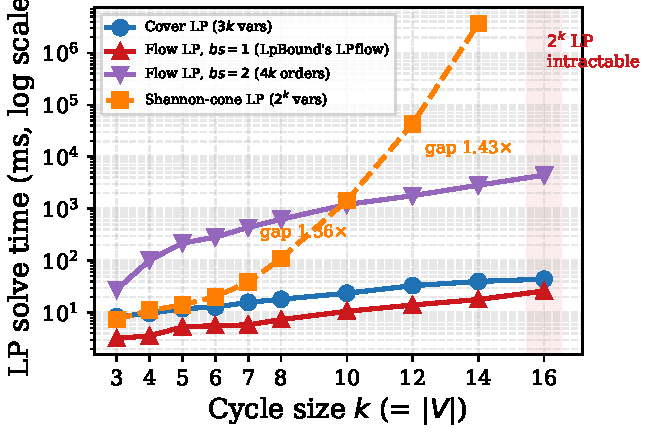
\includegraphics[width=\columnwidth]{crossover_entropic.pdf}
\caption{LP solve time on cycle-$k$ queries (log scale). The
Shannon-cone formulation of the $bs{=}1$ entropic bound grows
super-exponentially ($43$\,s at $k{=}12$, $3{,}679$\,s at $k{=}14$), but
LpBound's flow LP reaches the same bound (annotated gap to the cover LP)
in $3$--$26$\,ms. On $bs{=}2$ block statistics the flow LP over $4k$
orders takes $0.03$--$4.4$\,s and equals the $2^{|V|}$ polymatroid bound
at every even $k$ of this sweep. Data: \texttt{scale\_entropic.csv},
\texttt{flow\_scale.csv}.}
\label{fig:crossover}
\end{figure}

\paragraph{Choice of $p$-values.}
On cycle-6, using $\mathcal{P} = \{1,\infty\}$ (2 values) already
achieves $17.6\times$ improvement; adding $\ell_2$ ($\mathcal{P} =
\{1,2,\infty\}$) reaches $35.7\times$; further values ($\ell_3$,
$\ell_5$) yield no additional gain (Figure~\ref{fig:pvalue}).
We recommend $\mathcal{P} = \{1, 2, \infty\}$ as the default (cardinality
$\ell_1$, variance $\ell_2$, worst case $\ell_\infty$); repeating the
sweep on four families (cycle-4/6, $K_4$, chordal-5) confirms this is not
cycle-specific---$\ell_2$ helps in every family and $p$ beyond
$\{1,2,\infty\}$ adds $<2.4\%$.

\begin{figure}[t]
\centering
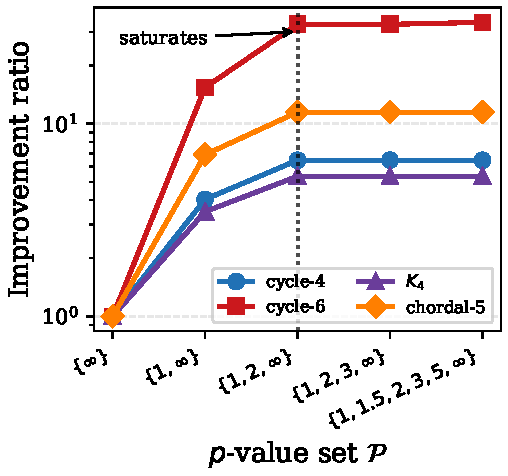
\includegraphics[width=\columnwidth]{pvalue_sensitivity.pdf}
\caption{Sensitivity to the number of $p$-values across four query
families (log scale). Improvement saturates at
$\mathcal{P} = \{1,2,\infty\}$ (dotted line) in every family;
additional norms add ${<}2.4\%$.}
\label{fig:pvalue}
\end{figure}

\subsection{WCOJ End-to-End Execution}

We evaluate ordering quality in a controlled GenericJoin
\emph{simulator} (a faithful Python implementation that counts
tuple-level iterations); the primary metric is the
\emph{iteration count}, which is deterministic and engine-independent,
while wall-clock time is reported as a single-machine reference and
varies $\pm 10\%$ across runs. To confirm the simulator computes the
correct join, we cross-validate its output cardinalities against
Ku\-zu---an independent WCOJ-capable graph engine---on cyclic patterns:
the counts match exactly across all tested configurations. A full
integration that \emph{injects} our ordering into a production engine is
left to future work; we found that neither DuckDB nor Ku\-zu exposes the
per-variable ordering hook this would require, so it entails modifying an
open-source WCOJ engine's planner.

\begin{table}[t]
\centering
\caption{WCOJ GenericJoin execution with different variable orderings.
LpH-CEG selects orderings that reduce intermediate result sizes.}
\label{tab:wcoj}
\begin{tabular}{@{}llrrr@{}}
\toprule
Query & Strategy & Iterations & Time (ms) & Speedup \\
\midrule
\multirow{2}{*}{Hetionet C-4}
  & Max-deg & 2,765,886 & 1,455 & $1.0\times$ \\
  & LpH-CEG & 1,209,687 &   560 & $\mathbf{2.6\times}$ \\
\midrule
\multirow{2}{*}{Cycle-4 synth.}
  & Max-deg &   258,068 & 1,063 & $1.0\times$ \\
  & LpH-CEG &   260,463 & 1,059 & $1.0\times$ \\
\midrule
\multirow{2}{*}{Triangle}
  & Max-deg &    38,757 &    72 & $1.0\times$ \\
  & LpH-CEG &    38,757 &    73 & $1.0\times$ \\
\bottomrule
\end{tabular}
\end{table}

Table~\ref{tab:wcoj} and Figure~\ref{fig:wcoj} demonstrate end-to-end
impact.
On the heterogeneous Hetionet cycle-4, LpH-CEG ordering
(gene1$\to$gene2$\to$compound$\to$disease) reduces iterations by
$2.3\times$ and simulator wall-clock time by $2.6\times$ versus
max-degree ordering
(compound$\to$disease$\to$gene2$\to$gene1).
The LP selects an ordering that processes high-selectivity joins first,
pruning intermediate results earlier.
On homogeneous synthetic data and acyclic queries, both orderings
perform identically, confirming that LP overhead does not harm
performance when improvement is unavailable.

\begin{figure*}[t]
\centering
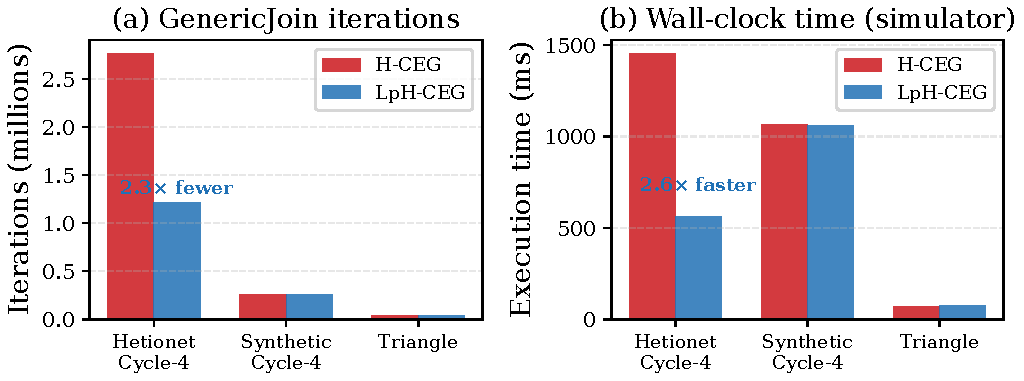
\includegraphics[width=0.85\textwidth]{wcoj_comparison.pdf}
\caption{WCOJ GenericJoin execution: (a)~number of tuple-level
iterations and (b)~wall-clock time.
LpH-CEG ordering reduces both by $2.3\times$/$2.6\times$ on
heterogeneous Hetionet joins, while matching max-degree on homogeneous
data.}
\label{fig:wcoj}
\end{figure*}

\subsection{End-to-End: Robustness of Bound-Guided Ordering}
\label{sec:robustness}

The WCOJ result above guides a multi-way join. We now ask the more
demanding systems question: can the cover bound guide \emph{binary} join
ordering inside a modern engine, and how does that compare to the
engine's own optimizer? We load each query into DuckDB, compute a
left-deep order by minimizing the classic $C_{\mathrm{out}}$
cost~\cite{leis2015goodare} (sum of the bound's estimated intermediate
cardinalities), inject it by disabling DuckDB's join-order optimizer, and
time real execution. As a reference we also run DuckDB's own
sampling-based optimizer.

Two honest findings frame the result. First, a cardinality \emph{upper
bound} is a conservative cost model: it never underestimates, so ranking
plans by it does not beat---and need not even match---an engine optimizer
on average. Second, and structurally, on a single cycle every proper
sub-query is acyclic, where the LP has no cyclic slack
(Proposition~\ref{prop:acyclic}), so the two bounds largely induce the
same order; the bound changes the ranking only when an
\emph{intermediate} sub-query is itself cyclic (cliques, chordal cycles).

What the pessimistic bound \emph{does} buy is robustness against
catastrophic plans. Table~\ref{tab:robust} reports, per query, each
strategy's slowdown over the best plan we found. DuckDB's optimizer is
excellent on average---often faster than any forced left-deep order
because it builds bushy plans---but on dense $4$-cliques its
sampling-based estimates badly underestimate the cyclic intermediate
blow-up, and it runs $7$--$21\times$ slower than optimal across every
clique density we tried. Bound-guided ordering, which by construction
cannot be lured into such a plan, stays within $3.6\times$ of optimal on
\emph{every} query in the suite. The worst-case (tail) slowdown is
$3.6\times$ for bound-guided versus $21\times$ for the engine---a
$5.9\times$ heavier tail for the sampling-based optimizer.

\begin{table}[t]
\centering
\caption{End-to-end robustness: slowdown over the best evaluated plan
(DuckDB, forced left-deep order vs.\ the engine's own optimizer).
Lower is better; the \emph{tail} row is the worst case over all queries.}
\label{tab:robust}
\begin{tabular}{@{}lrr@{}}
\toprule
Query & Bound-guided & DuckDB opt. \\
\midrule
Cycle-4 (100V/400E)        & $1.10\times$ & $0.60\times$ \\
Cycle-5 (100V/400E)        & $1.52\times$ & $0.14\times$ \\
$K_4$ clique (120V/800E)      & $1.64\times$ & $18.1\times$ \\
$K_4$ clique (120V/1500E)     & $3.32\times$ & $21.0\times$ \\
$K_4$ clique (120V/2500E)     & $1.81\times$ & $7.2\times$ \\
$K_4$ clique (200V/2000E)     & $1.57\times$ & $18.3\times$ \\
Diamond / chordal-4        & $2.54\times$ & $0.39\times$ \\
Chordal 5-cycle            & $2.11\times$ & $0.13\times$ \\
Hetionet $\triangle$ (real)& $3.56\times$ & $1.11\times$ \\
\midrule
\textbf{Worst case (tail)} & $\mathbf{3.6\times}$ & $\mathbf{21.0\times}$ \\
\bottomrule
\end{tabular}
\end{table}

\paragraph{The tail, over a broader distribution.}
Of six shapes at two sizes and three seeds, $24$ queries survive
(cycle-3/4, $K_4$, diamond; cycle-5 and chordal-5 censored entirely).
Medians are close ($1.03\times$ vs.\ $0.93\times$) while the tails
diverge: the bound-guided P95/max are $1.21\times$/$1.31\times$ against
DuckDB's $5.82\times$/$8.17\times$. Censoring uses the AGM bound, which
depends only on relation sizes---censoring by our own bound would drop
exactly the queries where it is loose. One caveat: the reference is the
best \emph{forced left-deep} order, so bound-guided is ${\ge}1$ by
construction while DuckDB, free to go bushy, scores below $1$ on median.
This shows a bound-guided choice avoids a plan space's tail, not that it
beats the engine.

\paragraph{Real data, block statistics.} The same protocol on the $40$
IMDb cycles at $|V|{=}6$, with four estimators behind $C_{\mathrm{out}}$,
tests the thesis rather than the $bs{=}1$ bound. Block statistics move the
choice toward the true-cardinality order: the flow LP on $bs{=}2$ picks
the order exact counts would pick on $24/40$ queries, and on the $33$
whose forced orders all finish within $60$\,s its median slowdown over the
best timed order (the strategies' picks plus $16$ sampled, of the $96$
connected left-deep orders) is $1.19\times$, against $1.41\times$ for the
$bs{=}1$ cover LP, $1.23\times$ for LpBound and $1.21\times$ for exact
counts---differences among the last three within noise. None competes with DuckDB's optimizer here ($0.43\times$
median, at most $2.0\times$): IMDb's cycles do not trigger its tail, and
on the other $7$ queries almost every forced left-deep order exceeds
$60$\,s while DuckDB finishes, so excluding them favors the forced
orders. A better bound improves \emph{which}
left-deep plan is chosen, not whether one should be.

This positions LpH-CEG honestly: it is not a replacement for a
well-tuned sampling optimizer, but a guide that bounds the worst case on
the dense cyclic queries that defeat sampling---on our synthetic cliques,
not on IMDb---consistent with the pessimistic-estimation rationale for
worst-case-optimal evaluation~\cite{cai2019pessimistic}.

\subsection{JOB, TPC-H, Data Size and Skew ($bs{=}1$)}
\label{sec:jobskew}

On the JOB-medium subset (CI: 3K, MK: 2K, MC: 1K rows) the two co-actor
4-cycles improve $1.94\times$ (with keywords) and $2.80\times$ (with
companies) at $bs{=}1$ with weights $w{=}0.5$, and a star query by
exactly $1.00\times$; the IMDb suite of Section~\ref{sec:suite} is the
systematic version. On TPC-H (SF${=}0.01$) every query yields
$1.00\times$: dimension keys such as \texttt{nation\_id} (25 values) are
near-uniform, and LpH-CEG needs both \emph{cyclic structure} and
\emph{degree skew}. On synthetic cycle-4 (10 seeds) the improvement grows
with data size, from $5.9{\pm}0.7\times$ at $100$ vertices to
$33.9{\pm}1.5\times$ at $2$K (relative std ${<}12\%$; a single-run sweep
reaches $57\times$ at $5$K), and peaks at moderate skew: $2.3{\pm}0.5\times$
at $\alpha{=}0.5$, $16.1{\pm}0.8\times$ at $\alpha{=}2.0$,
$6.6{\pm}0.4\times$ at $\alpha{=}3.0$. At low skew all $\ell_p$-norms
nearly coincide, at extreme skew $\ell_\infty$ is already near-tight, and
in between---the range real social and knowledge graphs
occupy~\cite{barabasi1999emergence}---$\ell_2$ captures the heavy tail.

\subsection{When LpH-CEG Does Not Help}
\label{sec:noimprove}

LpH-CEG yields no improvement ($1.00\times$) on (1)~acyclic queries---no
redundant coverage---and (2)~cycles of replicated relations with
near-symmetric sampled degrees (the $5$K-edge Epinions cycles,
Section~\ref{sec:realdata}); case~(2) is a property of the sample, as $20$K
edges of the same graph give $2.06\times$ on cycle-4
(Section~\ref{sec:suite}). What is required is \emph{asymmetric degree
structure in cyclic joins}. Synthetic power-law graphs improve more (up to
$614\times$ at cycle-8) than real data, where the median over the long
suites is $1.8$--$8.9\times$ (tails $157\times$ on Hetionet, $34\times$
on IMDb): Zipf skew at $\alpha\approx2$ exceeds real sub-linear degree
distributions and one $\alpha$ is shared by all relations.

%% ===================================================================
\section{Related Work}
\label{sec:related}

\paragraph{Block decomposition methods.}
CEG~\cite{salihoglu2026ceg} models pessimistic estimation as a shortest
path over single-relation max-degree weights; multi-way block
extensions~\cite{hceg2027} generalize this to groups of relations via
hyperpaths. Both use only $\ell_\infty$ statistics. LpH-CEG replaces the
scalar weights with LP-optimized $\ell_p$-norm products and
characterizes \emph{when} the LP can improve: cyclic queries with
redundant coverage (Theorem~\ref{thm:cyclic}).

\paragraph{Information-theoretic bounds.}
The AGM bound~\cite{atserias2008agm} uses fractional edge covers
with relation cardinalities ($\ell_1$-norms).
PANDA~\cite{abokhamis2017panda} and MOLP~\cite{joglekar2016molp} add
max-degree constraints ($\ell_\infty$-norms).
LpBound~\cite{zhang2025lpbound} generalizes to all $\ell_p$-norms,
showing that intermediate norms capture degree skew that max-degree
misses.
Two results since then bear directly on our reading. Im et
al.~\cite{im2025simple} compute the polymatroid bound for simple degree
constraints by a polynomial flow LP and prove the non-simple case
($|X|{\le}2$, $|Y|{\le}3$, the shape of a $bs{=}2$ block constraint)
hard, which is why our flow bound over blocks fixes an attribute order;
CorrBound~\cite{mayer2026corrbound} adds inner products of degree
vectors across join columns---a two-relation statistic in our
terms---to the entropic program and reports $6.7$--$16\times$ over
LpBound on cyclic queries. The first tightens inference at fixed
statistics, the second enriches statistics at fixed inference. The
$\ell_1$-norm of a $bs{=}2$ block sequence \emph{is} CorrBound's inner
product (the join size). In a proxy that adds exactly those sizes to the
entropic program, they are worth a median $31\times$ over LpBound on our
long suite, and the interface-conditioned block statistics a further
$63\times$ under the same program. The shared-interface block norms
$\sum_b \deg_R(b)^p\deg_S(b)^p$ are $\ell_p$-weighted inner products and
may fall within CorrBound's vocabulary; the one-side and common-neighbour
statistics do not, since they depend on \emph{which} values co-occur,
not only how often---and the latter needs the join that CorrBound's
sketches avoid (Section~\ref{sec:stats-vs-inference}).
Lin and Wang~\cite{lin2025ambidextrous} likewise tighten degree-sequence
bounds by counting claw \emph{pairs}, a richer statistic again.
SafeBound~\cite{deeds2023safebound} deploys degree-sequence bounds with
predicates on relational workloads, following pessimistic
CE~\cite{cai2019pessimistic}; we target graph patterns and a per-step
decomposition.

The entropy framework of Abo Khamis et al.~\cite{abokhamis2024lpnorm},
under which $\ell_p$-norm constraints are information inequalities, is
what Theorem~\ref{thm:composition} applies to block-joined relations.

\paragraph{Summaries and learned estimators.}
COLOR~\cite{deeds2025color} and PathCE~\cite{wang2025pathce} build
compact summaries; GNCE~\cite{schwabe2024gnce}, SPACE~\cite{aytimur2025space}
and FactorJoin~\cite{wu2023factorjoin} learn estimates. All produce
point estimates without a guarantee, for which pessimistic bounds are
the safety fallback~\cite{hceg2027}.

\paragraph{WCOJ algorithms.}
Yannakakis+~\cite{wang2025yannakakis} brings worst-case optimal joins to
DuckDB and PostgreSQL, a natural integration point for our ordering;
CompactLTJ~\cite{arroyuelo2025compactltj} shrinks Leapfrog Triejoin;
Capelli et al.~\cite{capelli2025simple} call for exactly the recursive
upper bounds our residuals provide---though our 66-query study shows
they do not beat max-degree ordering in general.

%% ===================================================================
\section{Practical Considerations}
\label{sec:practical}

\paragraph{When to use LpH-CEG.}
Use it on cyclic queries with $k \ge 4$ and moderately skewed data, with
$\mathcal{P} = \{1,2,\infty\}$; without a cycle, skip the LP. Degree
sequences can come from catalog histograms
($\lpnorm{\mathbf{d}}{p} = (\sum_i c_i d_i^p)^{1/p}$ over buckets
$(d_i, c_i)$) at \texttt{ANALYZE} time, on the filtered relation under
predicates. Optimizing $K{=}10$ candidate hyperpaths instead of one adds
$12.7$--$14.3\%$ on cycle-4 and $0\%$ on cycle-5.

\paragraph{Which block size to pay for.}
At $bs{=}1$, collecting degree sequences costs $22$--$27$\,ms against
${\sim}1.9$\,ms to solve. $bs{\ge}2$ multiplies that term by a median
$45\times$ ($24\times$ more entries, $9$--$19$\,MiB against
${\sim}0.3$\,MiB), once per database; cataloged, a $bs{=}2$ estimate
then costs $10$\,ms (Table~\ref{tab:long-suite}), and all but one
statistic per binary block need no join
(Section~\ref{sec:stats-vs-inference}). Use $bs{=}1$ when the bound is
re-solved many times per statistics build (per candidate order, per
prefix) and $bs{\ge}2$ when the pair joins can be materialized ahead of
the workload (the $\ell_2$ codegree norm needs them), solved by the flow
LP (Section~\ref{sec:scalability}) unless per-step residuals are
wanted.

%% ===================================================================
\section{Conclusion}
\label{sec:conclusion}

Replacing a max-degree product with a fractional cover LP is worth a
great deal---$654\times$ at cycle-8---but on single-relation statistics
little is left after it: on a fixed hyperpath the cover LP is optimal
over every valid weight vector, yet sits $1.25$--$1.43\times$ (synthetic)
and a median $2.5$--$4.3\times$ (real) above an entropic optimum that LpBound's
flow LP already reaches in polynomial time. The headroom is in the
statistics: block statistics are worth a median $56\times$ on short
Hetionet cycles, $80$--$2{,}500\times$ on longer ones and $4$--$43\times$
on IMDb ($17$--$177\times$ with the flow LP), below the entropic LpBound
on all $349$ cycle queries over real data and $12/12$ synthetic instances. Richer
statistics can reopen the program---on Hetionet and synthetic data the
optimum beats the cover LP by $1.5$--$5.1\times$ on them, on IMDb only
at scale ($6.8\times$ at $1{,}000$ films)---and a flow LP reaches that optimum in polynomial time
on synthetic even cycles and $189/240$ real-data queries.

We also state the limits. The separation is regime-dependent: on
homogeneous synthetic cycles the two axes are comparable; heterogeneous
real data splits them, and our evidence is binary graph patterns on two
real datasets (Hetionet, IMDb). Blocks cost a median $45\times$ more to collect, once per
database, and the one statistic that needs the join is the one that
matters; $30\%$ of the short Hetionet suite gains nothing at $bs{=}1$; the residual
ordering heuristic does not generalize; and upper bounds bias plans
conservative, so pairing them with optimistic estimators is the natural
next step. Even so, the question to ask of
a pessimistic estimator may be less which inequalities it uses than
which joins it will pay to materialize---and only then which program it
runs on them. We offer this as a characterization of where bound headroom
lies, not as a deployable optimizer: our queries are cycle patterns over
real data, of the kind subgraph-counting
work targets~\cite{deeds2025color,wang2025pathce}, our statistics come
from slices ($20$K rows, $200$--$1{,}000$ films) collected by a Python
prototype whose cost grew $11\times$ for $4.2\times$ the data, and full-scale
use needs the statistics cataloged inside the system.

%% ===================================================================
% ICDE 2027 requires disclosure of AI-generated content in the
% acknowledgments (IEEE policy); it does not count toward the 12 pages.
\section*{Acknowledgment}
\emph{Use of AI-generated content.} In accordance with the IEEE policy on
AI-generated content, we disclose that Claude (Anthropic), a large
language model used through the Claude Code tool, was used throughout this
work. It drafted and revised text in every section
(Sections~\ref{sec:intro}--\ref{sec:conclusion} and the abstract);
implemented and ran the experiment scripts behind
Sections~\ref{sec:experiments} and~\ref{sec:wcoj} and all tables; wrote
the first version of the proof of Theorem~\ref{thm:composition}; and
produced simulated reviews of drafts. Every number in the paper is
produced by the released scripts and checked against its source data by
an automated audit. The authors reviewed the content and take full
responsibility for it.

%% ===================================================================
\bibliographystyle{IEEEtran}
\bibliography{references}

\end{document}
